\documentclass[11pt]{article}
\usepackage[a4paper, margin=2.54cm]{geometry}

% español
\usepackage[spanish]{babel}

% imágenes
%\usepackage{graphicx}
%\graphicspath{{img}}

% fuentes de conjuntos numéricos
\usepackage{amsfonts}

% símbolos
\usepackage{amsmath, amssymb}

% gráficos
%\usepackage{tikz}

% plots
%\usepackage{pgfplots}
%\pgfplotsset{width=10cm, compat=1.9}

% shapes
%\usetikzlibrary{shapes.geometric}

% separación fórmulas en align
%\setlength{\jot}{8pt}

% espacio entre párrafos
%\usepackage[skip=10pt plus1pt, indent=12pt]{parskip}

% cancelar términos
\usepackage{cancel}

% links
%\usepackage[colorlinks=true, 
%    urlcolor=blue]{hyperref}

% incluir pdfs
%\usepackage{pdfpages}

% tipografía cheta
\usepackage{tgbonum}

% interlineado: 1.0 simple, 1.3 (1.5), 1.6 (doble)
\linespread{1.3}

\title{Física II\\Apuntes Khan Academy}
\author{Daniel Ise}
\date{Primer Cuatrimestre, 2025}

\begin{document}

\maketitle

\tableofcontents

\section{Carga eléctrica}

\subsection{Ley de Coulomb}

La fuerza ejercida entre cargas \(Q_1\) y \(Q_2\).

\vspace{1cm}
\begin{equation}
    F = k\frac{|Q_1Q_2|}{r^{2}}
\end{equation}
\vspace{1cm}

\begin{enumerate}
    \item Siendo F la fuerza entre las cargas (por tercera ley), medida en newton (N)
    \item \(k\) la \textbf{Constante de Coulomb} o \textbf{Constante electrostática},
    con valor aproximado 
    \begin{equation*}
        k_0\approx9\times10^{9} \frac{N\cdot m^{2}}{C^{2}}
    \end{equation*}
    \item \(Q_{1}\) y \(Q_{2}\) las cargas, medidas en coulomb (C)
    \item y \(r\) la distancia entre las mismas, medida en metros (m)
\end{enumerate}

La constante de Coulomb puede expresarse también como:

\vspace{1cm}
\begin{equation*}
    k_0 = \frac{1}{4\pi\epsilon_0}
\end{equation*}
\vspace{1cm}

Siendo \(\epsilon_0\) la \textbf{Constante de permitividad},
cuyo valor aproximado es: 
\begin{equation*}
    \epsilon_0 \approx 8.85 \times 10^{-12} \frac{C^{2}}{N\cdot m^{2}}
\end{equation*}.

\section{Campo eléctrico}

Es la fuerza potencial que una carga puede ejercer sobre una carga de prueba,
ubicada a un distancia \textit{r}.

\vspace{1cm}
\begin{equation}
    E = \frac{F}{Q_0} = k \frac{|Q|}{r^{2}}
\end{equation}
\vspace{1cm}

\begin{itemize}
    \item Siendo \(E\) el campo eléctrico, medido en \(\frac{N}{Q}\)
    \item \(F\) la fuerza que la carga \(Q\) puede potencialmente ejercer sobre la carga de prueba \(Q_0\)
    \item \(k\) la constante de Coulomb 
    \item \(r\) la distancia entre las cargas
\end{itemize}

\section{Flujo Eléctrico - Ley de Gauss}

Refiere al campo eléctrico que atraviesa una superficie de área \(A\).

\vspace{1cm}
\begin{equation*}
    \phi = E \cdot A \cdot \cos \theta
\end{equation*}
\vspace{1cm}

\begin{itemize}
    \item Siendo \(\phi\) el flujo eléctrico 
    \item \(E\) el campo eléctrico 
    \item \(A\) el área considerada
    \item \(\theta\) el ángulo entre el vector normal de la superficie y el vector del campo eléctrico
\end{itemize}

Cuando el vector normal de la superificie y el vector del campo eléctrico son paralelos,
\(\cos\theta = 1\), por lo cual la ecuación se reduce a:

\vspace{1cm}
\begin{equation}
    \phi = E\cdot A
\end{equation}
\vspace{1cm}

La ley de Gauss resulta de reemplazar \(E\) por \(k\frac{|Q|}{r^{2}}\) y,
a su vez,
\(k\) por \(\frac{1}{4\pi\epsilon_0}\).
Por otra parte,
el área considerada es la superficie de una esfera,
por lo cual \(A = 4\pi r^{2}\),
por lo cual llegamos a la expresión:

\vspace{1cm}
\begin{equation*}
    \phi = \frac{1}{4\pi\epsilon} \cdot \frac{|Q|}{r^{2}} \cdot 4\pi r^{2}
\end{equation*}
\vspace{1cm}

Simplificamos:

\vspace{1cm}
\begin{equation*}
    \phi = \frac{1}{\cancel{4\pi}\epsilon} \cdot \frac{|Q|}{\cancel{r^{2}}} \cdot \cancel{4\pi} \cancel{r^{2}}
\end{equation*}
\vspace{1cm}

Finalmente, llegamos a la expresión de la \textbf{Ley de Gauss}:

\vspace{1cm}
\begin{equation}
    \phi = \frac{|Q|}{\epsilon}
\end{equation}
\vspace{1cm}


\section{Unidad 2}

\subsection{Derivadas parciales}

La \textbf{derivada en un punto} \(P = (a,b)\),
de una función de una variable \(f(x)\),
devuelve la \textit{pendiente} \(m\),
de una recta que es tangente a \(f\) en el punto \(P\).

\vspace{.25cm}
\begin{equation*}
    \frac{df}{dx} = \lim_{\Delta x \to 0}\frac{\Delta y}{\Delta x} =
    \lim_{x \to a}\frac{f(x) - f(a)}{x-a}
\end{equation*}
\vspace{.25cm}

La derivada en funciones de dos variables sigue la misma idea:
aplicamos la derivada a cada una de las variables por separado,
considerando a la otra como constante.
Por eso hablamos de \textbf{derivada parcial}.

\begin{align*}
    \frac{\partial f}{\partial x} = f_x \\
    \\
    \frac{\partial f}{\partial y} = f_y \\
\end{align*}

Geométricamente,
podemos interpretar la derivada parcial respecto de \(x\)
en el punto \(P = (a, b, f(a,b))\),
como la \textit{pendiente} \(m\) de una recta tangente a la curva formada por
la intersección de \(f\) y el plano \(x = a\).
Lo mismo sucedería con la derivada parcial con respecto a \(y\).

\begin{figure}[H]
    \centering
    \caption{Interpretación geométrica de la derivada parcial}
    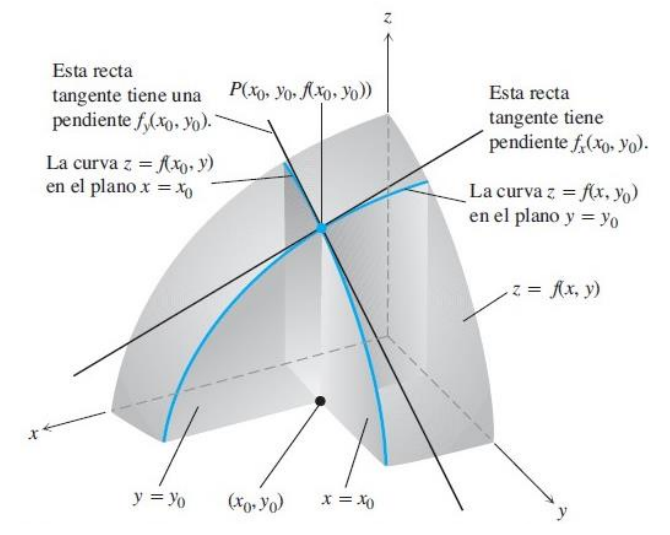
\includegraphics[scale=.8]{./img/01-02-derivada-parcial-geometrica.png}
\end{figure}

\vspace{.5cm}
\textbf{Ejemplo.}

Encontramos derivadas parciales de \(f(x,y) = x^{3} + x^{2}y^{3} - 2y^{2}\):

\begin{align*}
    f_x = 3x^{2} + 2xy^{3} \\
    f_y = 3x^{2}y^{2} - 4y \\
\end{align*}

\subsection{Propiedades y reglas de la derivada parcial}

\begin{enumerate}
    \item Con \(a\) constante:
          \begin{equation*}
              (a \cdot f)_x = a\cdot f_x
          \end{equation*}
    \item Distributiva respecto de la suma y resta:
          \begin{equation*}
              (f \pm g)_x = f_x \pm g_x
          \end{equation*}
    \item Regla del producto:
          \begin{equation*}
              (f\cdot g)_x = f_x\cdot g + f\cdot g_x
          \end{equation*}
    \item Regla del cociente:
          \begin{equation*}
              \left(\frac{f}{g}\right)_x = \frac{f_x\cdot g - f\cdot g_x}{g^{2}}
          \end{equation*}
    \item Regla de la cadena:
          Derivada parcial de \(g\), con \(f\) como está,
          por derivada parcial de \(f\):
          \begin{equation*}
              (g(f))_x = g(f)_x \cdot f_x
          \end{equation*}
\end{enumerate}

\subsection{Cálculo de derivada parcial por definición}

\subsubsection{Cuando la derivada no es continua en un punto}

Calculamos por definición,
manteniendo una constante.

\vspace{.5cm}
\textbf{Ejemplo.}

Calcular derivadas parciales de \(\sqrt[3]{x^{3} + y^{3}}\) en el origen:

Si calculamos derivada directamente:
\begin{align*}
    f_x & = \frac{1}{3}(x^{3} + y^{3})^{-2/3} \cdot 3x^{2} \\
    f_x & = \frac{x^{2}}{\sqrt[3]{(x^{3} + y^{3})^{2}}} \\
\end{align*}

Si evaluaramos esta derivada parcial en el origen,
encontraríamos una indeterminación.
Sin embargo, 
si derivamos por definición en el punto:

\begin{align*}
    f_x & = \lim_{x \to 0}\frac{f(x,0) - f(0,0)}{x - 0} \\
    f_x & = \lim_{x \to 0} \frac{\sqrt[3]{x^{3}} - 0}{x} \\
    f_x & = \boxed{1} \\
\end{align*}

Vamos con \(f_y\):

\begin{align*}
    f_y & = \lim_{y \to 0}\frac{f(0,y) - f(0,0)}{y - 0} \\
    f_y & = \lim_{y \to 0}\frac{y - 0}{y - 0} \\
    f_y & = \boxed{1}
\end{align*}

Aproximándonos por los ejes \(x\) e \(y\) la derivada tiende a \((1,1)\).


\subsubsection{Cuando está definida por partes}

Donde se da el cambio de función la derivada debe evaluarse por definición.

\vspace{.5cm}
\textbf{Ejemplo.}

Calcular derivada de:
\begin{align*}
    \begin{cases}
        \frac{3xy}{x^{2} + y^{2}} & (x,y)\neq (0,0) \\
        0 & (x,y) = (0,0)
    \end{cases}
\end{align*}

Calculamos por definición donde se produce el cambio de función:

\begin{align*}
     f_x & = \lim_{h \to 0}\frac{f(0 + h,0) - f(0,0)}{h} \\
     f_x & = \lim_{h \to 0}\frac{0 - 0}{h - 0} = \boxed{0} \\
\end{align*}

\begin{align*}
     f_y & = \lim_{h \to 0}\frac{f(0,0 + h) - f(0,0)}{h - 0} \\
     f_y & = \lim_{h \to 0}\frac{0 - 0}{h - 0} = \boxed{0} \\
\end{align*}

La derivada parcial respecto de \(x\) y respecto de \(y\) en \((0,0)\) valen 
ambas 0.

\subsubsection{Cuando puede que una exista y la otra no}

\subsubsection{Derivabilidad y continuidad}

En funciones de una variable la derivabilidad implica continuidad:
si una función es derivable en el punto \(P\),
se puede afirmar que es continua en \(P\).

Lo recíproco, siempre en funciones de una variable,
no se puede asegurar:
que una función sea continua no implica que sea derivable.
El ejemplo clásico es la función \(f(x) = |x|\). 
Esta función no es derivable en \(x = 0\),
puesto que la derivada por izquierda es distinta de la derivada por derecha.

Sin embargo,
en funciones de varias variables,
la derivabilidad \textit{no implica} continuidad.
Por ejemplo, la función \(\frac{3xy}{x^{2} + y^{2}}\).
Sus derivadas parciales en \(x\) y \(y\),
determinadas por definición,
son iguales a 0.
Pero esta función claramente \textit{no es continua} en 0.

Derivabilidad, 
en funciones de varias variables,
no implica continuidad.

\subsection{Derivadas de orden superior o derivadas sucesivas}

Una función de 2 variables independientes tiene \(2^{2}\) 
derivadas de 2\(^{\circ}\) orden:

\begin{align*}
    f_{xx} \quad f_{xy} \quad f_{yy} \quad f_{yx}
\end{align*}

Generalizando,
una función de \(m\) variables tiene \(m^{n}\) derivadas de \(n\) orden.

La notación de las derivadas de segundo orden es:

\begin{equation*}
    f_{xy} = \frac{\partial^{2} f}{\partial y \partial x} \quad 
    f_{xx} = \frac{\partial^{2} f}{\partial x^{2}}
\end{equation*}

\subsection{Teorema de Schwarz}

Si existen en torno al punto \(P\) \(f_x\),
\(f_y\)
y \(f_{xy}\),
con \(f_{xy}\) continua en \(P\),
\textbf{existe} \(f_{yx}\) y \(f_{yx}|_P = f_{xy}|_P\).

En concreto,
las derivadas cruzadas son iguales 
en todos los puntos del dominio donde sean continuas.

\vspace{.5cm}
\textbf{Ejemplo.}

Hallar derivadas de segundo orden de \(f(x,y) = x \cos y + ye^{x}\):

Hallamos primero derivadas de primer orden:

\begin{align*}
    f_x = \cos y + ye^{x} \quad f_y = -x\sen y + e^{x}
\end{align*}

Buscamos las derivadas de segundo orden:

\begin{align*}
    f_{xy} = -\sen y + e^{x} \quad f_{yx} = -\sen y + e^{x}
\end{align*}

Vemos que ambas son continuas,
por lo cual se cumple el Teorema de Schwarz:
las derivadas cruzadas son iguales.

\subsection{Dos matrices especiales}

\subsubsection{Matriz jacobiana}

Es una matriz \(m \times n\),
cuyas filas son las derivadas parciales de \(m\) funciones,
de \(n\) variables.

Por ejemplo, una matriz jacobiana de dos funciones \(f\) y \(g\),
de dos variables, sería:

\begin{equation*}
\BIG{J =
    \begin{pmatrix}
        \frac{\partial f}{\partial x} & \frac{\partial f}{\partial y} \\
        \frac{\partial g}{\partial x} & \frac{\partial g}{\partial y} \\
    \end{pmatrix}}
\end{equation*}

\subsubsection{Matriz Hessiana}

Matriz de las derivadas parciales \textit{de 2do orden}
de \textit{una} función.
Por ejemplo, la hessiana de una función de 2 variables sería:

\begin{equation*}
\BIG{H =
    \begin{pmatrix}
        f_{xx} & f_{xy} \\
        f_{yx} & f_{yy} \\
    \end{pmatrix}}
\end{equation*}

\subsection{Regla de la cadena}

Si \(f(x,y) = z\),
y podemos expresar x e y en función de t,
es decir, \(x(t)\) e \(y(t)\),
se puede hacer una composición \(z(t)\).

Se puede componer y derivar \(\frac{dz}{dt}\) o, por regla de la cadena:

\begin{equation*}
    \frac{dz}{dt} = \frac{\partial z}{\partial x}\cdot\frac{dx}{dt} + \frac{\partial z}{\partial y}\cdot\frac{dy}{dt}
\end{equation*}

Ahora, 
supongamos \(z = f(x,y)\),
que a su vez \(x = x(u,v)\) e \(y = y(u,v)\).
En este caso,
\(z\) tendrá una derivada parcial respecto de \(u\)
y una derivada parcial respecto de \(v\),
siguiendo la estructura del punto anterior:

\begin{align*}
    z_u = f_x\cdot x_u + f_y \cdot y_u \\
    z_v = f_x\cdot x_v + f_y \cdot y_v \\
\end{align*}

\subsection{Derivada direccional}

Ya hemos visto las derivadas parciales,
que son las tasas de cambio de \(z\) en dirección de los ejes \(x\) e \(y\).

La derivada direccional es la tasa de cambio del campo vectorial en dirección 
de un vector \(\vec{u}\).

El vector \(\vec{u}\) puede definirse básicamente de dos maneras:
\begin{itemize}
    \item Con \textbf{puntos} \(a\) y \(b\), 
    que para referir el vector al origen los restamos \(\vec{u} = b-a\)
    \item Con el \textbf{ángulo} \(\theta\),
    de forma \(\vec{u} = (\cos \theta, \sen \theta)\).
\end{itemize}

Para realizar una derivada direccional el vector debe estar normalizado.
Un vector dado por su ángulo \textit{ya se encuentra normalizado}.
Para normalizar un vector dado por sus puntos operamos:

\begin{equation*}
    \vec{n} = \frac{\vec{u}}{|\vec{u}|}
\end{equation*}

Siendo la magnitud del vector \(|\vec{u}| = \sqrt{a^{2} + b^{2}}\).

Dado el punto \(P = (x_0, y_0, z_0)\), 
la derivada direccional en dirección de \(\vec{u} = (a,b)\) es:

\begin{equation*}
    D_{\vec{u}}f(x,y) = \lim_{h \to 0}
    \frac{f(x_0 + ha, y_0 + hb) - f(x_0,y_0)}{h}
\end{equation*}

\textbf{Teorema de la derivada direccional.}

Si \(f\) es diferenciable en \(P = (x_0,y_0)\),
entonces tiene derivada direccional en sentido de cualquier vector 
\(\vec{u} = (a,b)\), donde:

\begin{equation*}
    D_{\vec{u}}f(x,y) = f_x|_{P} \cdot a + f_y|_{P} \cdot b
\end{equation*}

\textbf{Ejemplo.}

Hallar derivada direccional de \(f(x,y) = x^{3} - 3xy + 4y^{2}\),
en dirección de \(\vec{u}\) con \(\theta = \pi/6\).
Determinar valor de la razón de cambio siguiendo ese vector en \(P = (1,2)\).

Instrucciones:
\begin{itemize}
    \item Primero especificamos/normalizamos el vector
    \item Calculamos derivadas parciales 
    \item Planteo el teorema de la derivada direccional 
    \item Obtengo una expresión
    \item Evaluamos en \(P\)
    \item Llegamos al valor
\end{itemize}
\section{Materiales aislantes y materiales conductores}

Los materiales se pueden clasificar,
a grandes rasgos,
en aislantes y conductores\footnote{Aunque hay más tipos de materiales, como los semiconductores y los superconductores, a grandes rasgos y para este nivel de física podemos quedarnos con estos dos}.

Tienen en común su \textbf{cantidad enorme} de átomos y moléculas,
ambos con carga positiva en el nucleo y carga negativa en los electrones alrededor.
Además en ambos,
siempre que sean sólidos,
los núcleos no se van a poder mover libremente,
solo se pueden mover los electrones.

Su diferencia empieza precisamente en el movimiento de los electrones:
en los conductores los electrones se mueven con relativa facilidad,
por todo el material.
En los aislantes pueden pasar de un átomo a otro,
pero no con libertad.

A simple vista,
podría parecer que los conductores son mas relevantes,
pero esto no es así.
Aunque las cargas no floten,
los aislantes puede interactuar eléctricamente,
por ejemplo agregando cargas eléctricas
(como en el caso del globo visto en el primer punto).

En un conductor,
si agregamos cargas extras,
estas se acumulan en la parte exterior,
se mueven hacia su superficie.
Como los electrones gozan de libertad,
al repelerse entre si tienden a distribuirse uniformemente 
en los puntos más alejados entre sí.
Esos puntos son la superficie del conductor.

Ejemplos de materiales aislantes son vidrios, maderas, plásticos.
En los conductores incluimos metales como el oro, cobre, plata.

\subsection{Carga de un conductor por inducción}

Si acercamos un material cargado negativamente a un conductor neutro,
sus cargas negativas tenderán a desplazarse al lado contrario al material.
Si conectamos el conductor a \textit{tierra}
-que podemos imaginar como un resumidero infinito-
los electrones fluirán hacia ella,
cargando al conductor positivamente.
Luego de retirar la conexión a tierra,
hemos cargado al conductor positivamente \textit{por inducción}.

\section{Ejercicio 4}

\begin{figure}[H]
    \centering
    \begin{circuitikz}[american voltages]
        % componentes:
        \draw 
            (0,0) 
            to     (6,0)
            to [C,l_=$100\mu F$]                     (6,4)
            to [R,l_=$1k\Omega$]                     (0,4)
            to [battery1,l_=$10V$] (0,0);
    \end{circuitikz}
\end{figure}

La fórmula de carga del capacitor sigue la expresión
\(V_C=V_0(1-e^{-t/RC})\);
donde \(V_C\) es tensión en tiempo \(t\),
medida el \textit{volts} \((V)\);
\(V_0\) es tensión final o máxima;
\(e\) es el número de Euler;
\(t\) es el tiempo,
en \textit{segundos} \((s)\);
\(R\) es resistencia,
medida en \textit{ohms} \((\Omega)\);
\(C\) es capacitancia,
medida en \textit{faradios} \((F)\);
notar que \(RC\) se conoce como 
constante de tiempo,
que indica la rapidez de carga o descarga del capacitor,
representada por \(\tau\),
y se mide en \textit{segundos} \((s)\).

¿Cuál es la tensión de carga en \(t=0\)?
¿En \(t=0.1s\)?
¿Y en \(t=\infty s\)?

En 0 y en \(\infty\) resolvemos deduciendo:
0 y \(10V\), respectivamente.
Operamos para calcular en \(0.1s\):

\begin{align*}
    RC &= 100\times10^{-6}F \cdot 1\times10^{3} \Omega \\
    RC &= \boxed{0.1}
\end{align*}

Por lo tanto:

\begin{align*}
    V_C = 10V \cdot (1-e^{-0.1/0.1}) \\
    V_C = \boxed{6.32V}
\end{align*}
\section{Clase 16 de mayo}

\subsection{}

\section{Dirección del campo eléctrico}

\begin{enumerate}
    \item Encontrar dirección del campo eléctrico
    \item Encontrar dirección de la fuerza
\end{enumerate}

Por convención,
para definir un campo eléctrico usamos una carga de prueba positiva,
de manera tal que el campo eléctrico apunta 
en la misma dirección que la fuerza eléctrica.

En otras palabras,
si la carga de origen es positiva,
la fuerza eléctrica ejercida sobre la carga de prueba apuntará hacia afuera,
puesto que ambas son positivas.
El campo eléctrico apunta hacia afuera.

Si cambiamos la carga de prueba de posición,
vemos que el vector de fuerza tendrá siempre dirección radial hacia afuera 
de la carga de origen.

En cambio,
si la carga de origen es negativa,
la dirección de la fuerza sobre la carga de prueba será radial 
y hacia el centro del campo.
El campo eléctrico originado por una carga negativa apunta hacia su centro.

Lo potente en la idea del campo eléctrico es que puedo 
\textit{abstraer} su origen:
a eso se refiere con \textit{localidad},
que es una cualidad buscada en física.

Entonces,
si la carga de prueba es positiva,
la fuerza eléctrica ejercida sobre ella apunta en la misma dirección.
Si tenemos una carga de prueba negativa,
la fuerza eléctrica apunta en dirección contraria al campo eléctrico.

Por ello decimos:
1. encontramos dirección del campo eléctrico,
2. encontramos la dirección de la fuerza eléctrica.

\section{Clase 22 de mayo - Segunda mitad}

\subsection{Ingreso nacional}

(Introducción al Producto Interno Bruto)

Los economistas suelen utilizar información estadística
para evaluar la evolución de la economía.
En general, la información económica se expresa en unidades monetarias.
Básicamente,
se trata de hacer un relevamiento y registro de una serie de magnitudes,
de variables,
referidas a transacciones económicas en un período dado.

\subsection{Sectores productivos de la economía}

Se denomina sector al conjunto de unidades productivas que actúan en la economía,
que tienen en común ciertas características referidas al tipo de bienes que producen
o a las tecnologías que utilizan:

\vspace{.5cm}
\begin{table}[H]
    \centering
    \begin{tabular}{ll}
        \hline
        Sector primario   & Agricultura, minería pesca \\
        Sector secundario & Industria manufacturera    \\
        Sector terciario  & Servicios                  \\
        \hline
    \end{tabular}
\end{table}
\vspace{.5cm}

A su vez cada uno de los sectores puede subdividirse en varios otros,
dando lugar así a una clasificación más detallada.
Por ejemplo,
en el sector secundario puede haber distintas ramas industriales,
como la alimentaria, la química,
la metalúrgica,
etc.

También estas subdivisiones se pueden,
a su vez,
dividir en otros componentes,
como la alimentaria en vitivinícola,
aceitero,
lácteos,
conservas,
etc.

\subsection{Factores de producción y remuneración percibida}

\vspace{.5cm}
\begin{table}[H]
    \centering
    \begin{tabular}{ll}
        Factores & Remuneración     \\
        \hline
        Trabajo  & Salario o sueldo \\
        Capital  & Interés          \\
        Tierra   & Renta            \\
        Empresa  & Beneficios       \\
        \hline
    \end{tabular}
\end{table}
\vspace{.5cm}

El factor genera o recibe una remuneración.

Para producir intervienen cuatro elementos o factores.
La producción resulta de la articulación del trabajo, el capital, la tierra y la empresa.
En la práctica,
muchas veces suelen confundirse las remuneraciones de alguno de los factores entre sí.
¿El dueño de una empresa recibe beneficio o salario?

Por ejemplo,
si hablamos de la tierra,
el dueño al explotarla está recibiendo dos tipos de beneficios en uno:
la ganancia por cultivar y la renta que ganaría si hubiese dado en alquiler.
El empresario recibe dos rentas como beneficio de la empresa:
una como si tuviera un sueldo que le paga su propia empresa
y la otra el adicional por su riesgo empresarial.

\subsection{Clasificación de bienes disponibles}

Los bienes pueden clasificarse según el uso que se haga de ellos en el proceso económico,
como por ejemplo,
bienes finales y bienes intermedios.

\begin{itemize}
    \item Finales
          \begin{itemize}
              \item No durables
              \item Durables
                    \begin{itemize}
                        \item De consumo
                        \item De producción
                    \end{itemize}
          \end{itemize}
    \item Intermedios
\end{itemize}

\textbf{Bienes durables de producción:} Son aquellos que se destinan a producir otros bienes.

\textbf{Bienes intermedios:}
Son aquellos que no se usan ni para producir ni para consumir
en el estado en que se encuentran,
sino que son utilizados en el proceso productivo
destinado a producir otros bienes.
Ejemplo:
Para el pan se utiliza harina.
El pan es un bien final.
El trigo y la harina,
en este caso,
es un bien intermedio.
\section{Clase 23 de junio}

\subsection{Presentaciones de trabajos de investigación}

Hoy continua la presentación de trabajos de investigación.
El tema que voy a dar es \textbf{reingeniería}.

Hay que preparar diapositivas.
\section{Clase 27 de junio}

\subsection{Ejercicio 1}

Revisar foto.

\subsection{Ejercicio 2}

Fuente de \(f = 60 Hz\), resistencia de \(50 mHz\).
Si reactancia es \(X_L = 2\pi f L\), entonces:

\begin{align*}
    X_L = 2\pi \cdot 60 \cdot 50 \times 10^{-3}
    \boxed{X_L = 18.85 \Omega}
\end{align*}

\subsection{Ejercicio 3}

Si \(\epsilon = B\cdot l \cdot v\),
con 

\subsection{Ejercicio 4}

Tenemos un circuito, con pila de \(10V\)

Si velocidad de carga \(V_C = V_0(1-e^{-\frac{t}{RC}})\),
¿Cuál es la tensión de carga en 0s? ¿En \(0.1\)? ¿En \(\inf\)?

En 0, la carga será \(\boxed{0 V}\).

En \(0.1\), la carga será:

\begin{align*}
    
\end{align*}

En \(\inf\) la carga tiende a \(10 V\).

\subsection{Ejercicio 5}


\section{Clase 12 de junio}

\subsection{Incoterms}

Son reglas para la implementación de los términos comerciales
fijados por la cámara de comercio internacional. 
La palabra \textit{incoterms} es una contracción,
que significa International Commercial Terms
(Términos de comercio internacional).

Los incoterms se centran en la obligación de entrega desde el punto de vista del
\textit{vendedor} (el exportador).

Los incoterms regulan:
\begin{itemize}
      \item La distribución de documentos
      \item Las condiciones de entrega de la mercadería
      \item La distribución de costos de la operación
      \item La distribución de riesgos de la operación 
\end{itemize}

Pero \textbf{no} regulan:
\begin{itemize}
      \item La legislación aplicable
      \item Las formas de pago de la operación 
\end{itemize}

Así pues, 
los incoterm definen y reparten claramente las obligaciones, 
los gastos, 
los riesgos del transporte internacional 
y el seguro tanto en el exportador como el importador.

El incortem seleccionado entre el exportador y el importador
determinará quien pagará el costo de cada segmento del transporte,
quién será responsable de cargar y descargar la mercadería,
y quién lleva el riesgo de la pérdida en un momento dado durante el envío
(sea local o internacional).

Se clasifican en dos grupos fundamentales:
\begin{enumerate}
      \item Grupo de salida
      \item Grupo de llegada
\end{enumerate}

\textbf{Grupo de salida.}
Empiezan con la letra E, F, C.

\textbf{Grupo de llegada.}
Empiezan con la letra D.

A comienzos del siglo XX,
se estableció la necesidad de la reglamentación del contrato de compraventa 
internacional,
y fue así que se crearon en 1936,
habiendo varias revisiones o endosos posteriores.

\subsection{Ejemplos de los principales términos incoterms}

\textbf{Grupo de salida.}
\begin{itemize}
      \item EXW: Exwork el vendedor entrega el producto en la puerta de su fábrica. 
      De ahí en adelante el resto de gastos corren por cuenta del comprador.
      \item FAS: Free Alongside Ship (franco al costado del buque).
      La entega de la mercadería se realiza cuando es colocada por el vendedor 
      al costado del buque en el puerto de carga. Desde ahí, todos los costos 
      y riesgos quedan a cargo del comprador.
      \item FOB: Free On Board (franco abordo).
      El vendedor tiene la obligación de cargar la mercadería a bordo del buque 
      en el puerto de embarque y el comprador de encarga del resto 
      (Seleccionar el buque, contratarlo, pagar el flete marítimo,
      el seguro, los gastos de descarga, aduana y flete en destino).
      \item CFR: Cost and Freight (Costo y Flete).
      El vendedor paga los gastos de transporte y otros para que la mercadería 
      llegue al puerto convenido en destino. Incluye también el despacho 
      (aduana) de la mercadería de exportación. Pero el seguro del buque va a 
      cargo del comprador.
      \item CIF: Cost, Insurance and Freight (Costo, seguro y flete).
      Igual al anterior, pero el vendedor se hace cargo del seguro 
      internacional.
\end{itemize}

\textbf{Grupo de llegada.}
\begin{itemize}
      \item DAF: Delivered at frontier (entregado en frontera)
      El vendedor cumple su obligación de entregar la mercadería hasta un punto
      convenido de la frontera antes de rebasar la aduana.
      \item DDP: Delivered duty paid (entregado con pago de derechos)
      En este término el vendedor realiza la entrega de la mercadería al 
      comprador ya con el despacho terminado de importación en la puerta del 
      lugar convenido del país importador (el vendedor se encarga de todo).
\end{itemize}

En el transporte internacional,
los recibos de embarque de las mercaderías toman 
diferentes nombres de acuerdo al medio de transporte.
\begin{enumerate}
      \item Conocimiento de embarque o Bill of Lading (BL). Es el documento por 
      medio del cual se instrumenta el contrato de transporte de mercadería 
      por agua. No indica el precio de la mercadería, es simplemente un recibo,
      no es una factura. El BL es entregado por el transportador, por lo cual 
      acredita el contrato de transporte.
      \item Vía aérea, Air Waybill (AW). (Igual al primero)
      \item  Guías Aéreas (Air Waybill): 
      \item Carta de Porte: 
      se utiliza en transporte terrestre internacional. 
      Recibo de carga con la descripción de la mercadería.
\end{enumerate}

\end{document}